%%%%%%%%%%%%%%%%%%%%%%%%%%%%%%%%%%%%%%%%%%%%%%%%%%%%%%%%%%%%%%%%%%%%%%%%%%%%%%%%
\section{Future Work}
%%%%%%%%%%%%%%%%%%%%%%%%%%%%%%%%%%%%%%%%%%%%%%%%%%%%%%%%%%%%%%%%%%%%%%%%%%%%%%%%
\label{sec:future}

As Landslide is an experimental foray into the world of systematic exploration in kernel-space, and a detailed study of systematic exploration in general, it has opened up many avenues for potential future improvements.

\subsection{Interface Improvements}
\label{sec:future-interface}

Through our evaluation, we found many ways in which Landslide's user interface is lacking. These improvements would not be research developments, but would enhance the user experience in ways necessary for continuing work in the context of 15-410.\footnote{
Landslide is also missing functionality to automatically identify decision points when newly-forked threads become runnable but not immediately switched to. This was not necessary to find the \texttt{double\_thread\_fork} bug in POBBLES (Section~\ref{sec:eval-casestudy}) only because POBBLES automatically switched to the child thread immediately.}

\begin{itemize}
	\item Landslide currently does not support ability to replay a particular choice sequence. If the user finds a bug, and wants to re-execute the interleaving that led to it, they have no choice but to re-explore the tree.
	\item Landslide currently does not support being interrupted, so the user can use the Simics debug prompt arbitrarily and resume Landslide when ready. This is because the current implementation uses a wrapper script around the Simics prompt which Landslide communicates with to perform backtracking; it would be difficult to redesign, but could also be worked around.
	\item Landslide could print its decision traces in a better format. The current format is basically a ``raw data dump''. Raw text is probably the wrong interface; a graphical/tabular format with distinct columns for the execution of each different thread would be easier to understand.
\end{itemize}

\subsection{Education}
\label{sec:future-education}
% teaching tool, study thinking patterns
% 410 stuff
% TODO

\begin{figure*}[h]
	\begin{center}
	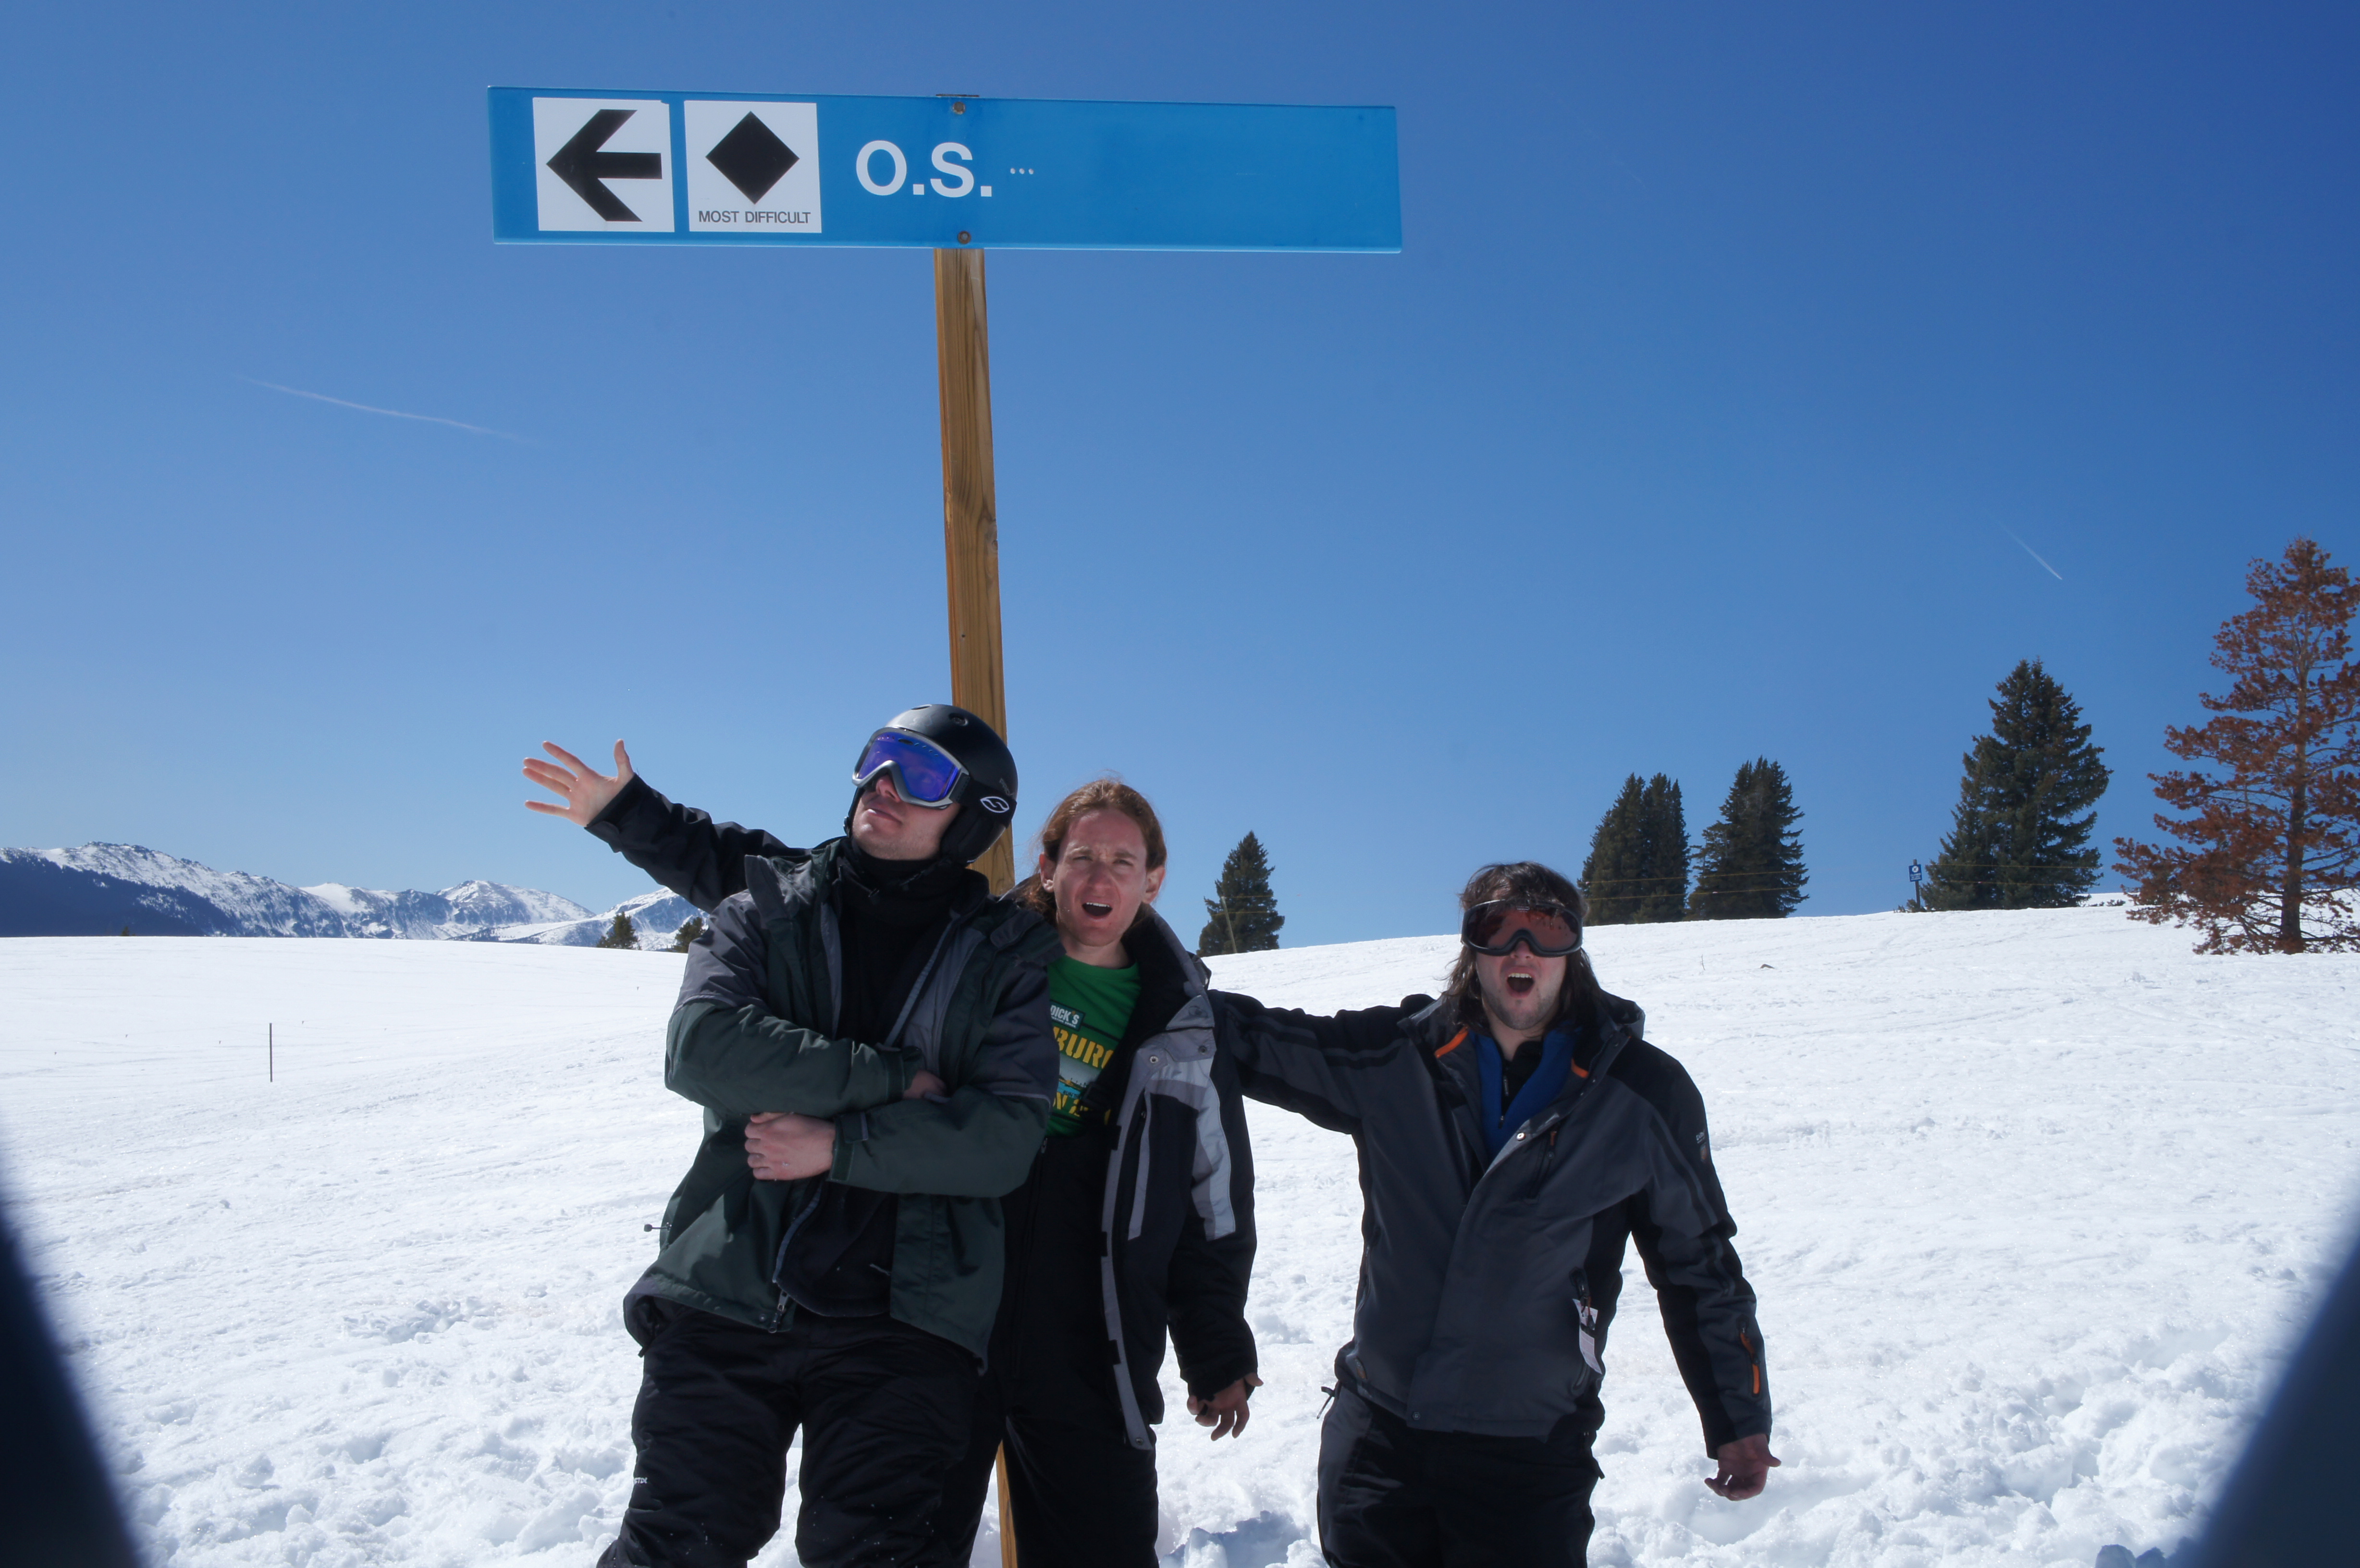
\includegraphics[width=0.75\textwidth]{wont-modify-vail.jpg}
	\end{center}
	\caption{Ex-members of Operating Systems course staff lament the difficulty involved in teaching students concurrency debugging skills.}
\end{figure*}

15-410 currently teaches students concurrency debugging skills ``the hard way'': by immersing them in environments where races will arise, and letting them find debugging tactics to use in conjunction with conventional stress testing on their own.

\subsection{New Techniques}
\label{sec:future-new}

Related research in dynamic verification has introduced testing techniques orthogonal to systematic exploration, which could augment its effectiveness if combined in one tool. We discuss the potential for using other techniques in Landslide or in any other systematic testing framework.

\subsubsection{Data Race Detection and Static Analysis}
\label{sec:future-analysis}

Landslide currently never alters its set of decision points once it begins executing. The user must configure the set of decision points in advance, and Landslide follows them to the letter when exploring the tree. This is useful for investigating the size of trees generated by certain sets of decision points, but future work should do better than leaving it up to the user to stumble across a set of decision points that exposes a bug.

Most notably among the information Landslide has at its disposal is the collection of conflicting shared memory accesses among transitions. Theoretically, to identify a decision point immediately before and after each such access would generate an execution tree with perfect granularity (i.e., exactly one shared memory access per transition), and thence find every possible race condition - this is, of course, the opposite extreme to the current setup.

Landslide could make use of data race detection techniques\cite{datacollider}, however, to strike a middle ground in which shared memory accesses it chooses.
\begin{enumerate}
	\item It should be aware of the types and interfaces associated with the kernel's synchronisation primitives (mutexes, condvars, semaphores, etc), and be able to treat operations on those as ``guaranteed to work'' (similar to Section~\ref{sec:por-independence}).
	\item Next, it should recognise acquire and release (or sleep and wake) operations on synchronisation primitives, and use that information to track lockset-type information.
	\item Ultimately, it should use the lockset information in conjunction with the happens-before relation to identify which memory accesses are ``raciest'', and add decision points around those.
\end{enumerate}

There may also exist static analysis techniques that would identify the most "at-risk" memory accesses, which could also be used in this manner.

\subsubsection{Parallelism}

Landslide's tree exploration is implemented sequentially. However, because DPOR's approach of tagging which sibling branches should be explored next generally follows a workqueue-based depth-first-search structure, it should not be too difficult to parallelise. Prior work exists for this technique\cite{distributed-dpor}, so it would not be a research contribution, but would substantially improve Landslide's effectiveness regardless.

\subsubsection{Symbolic Execution}
% TODO
symbolic execution\cite{klee,dawson}

\subsubsection{Trace Minimisation}
% TODO
% \ref{sec:future-backwards}

\subsection{Production Kernels}
\label{sec:future-linux}
% linux, device drivers
% open-coded sync dances: UGH (ad-hoc yield loops would make landslide get stuck)
% embedded microcontroller operating systems, simulated


\subsection{Performance}
\label{sec:future-perf}
% VM instead of simics
% - how to interpose? single-step, or unmap heap, and/or annotate (for hooks) with hypercalls
% - how to time travel? instead of time travel, snapshot once and replay

\subsection{Long-Running Testing Approaches}
\label{sec:future-shaping}

% TODO more
\subsubsection{Iterating Decision Sets}

In Section~\ref{sec:discussion-strategies}, we recommend an iteration strategy to effectively explore trees with multiple different sets of decision points, while not knowing ahead of time which, if any, may contain a bug.
This strategy would give rise to a test framework which could explore multiple different types and granularities of interleavings at once, heuristically judge which are more likely to uncover bugs, and prioritise resource allocation and search direction accordingly.

There is also the question of when during the testing process new decision points should be introduced.
One possibility would be to begin exploration with a small set of decision points, explore the resulting tree, analyse the tree post-hoc to identify additional decision points, and iterate exploring with the new set.
Another possibility would be to identify decision points along the way, analysing each branch of the tree after executing it, to generate the decision points for that very branch, and thence use them to find which branch to explore next.
It remains to be seen which approach would be more effective.

\subsection{Theoretical Oddities}
\label{sec:future-theory}
% theory things to study:

% TODO: make visualisations for both of these
\subsubsection{``Backwards'' Exploration}
\label{sec:future-backwards}
% - study the implications of backwards vs forward exploration
% - ICB as in chess

\subsubsection{Exploration Tree Structure}
% - nadim's backtrack depth
